\section{Comparison with HL-LHC PDF projections}
\label{app:comparisons_with_HLLHC}

%%%%%%%%%%%%%%%%%%%%%%%%%%%%%%%%%%%%%%%%%%%%%%%%%%%%%%%%%%%%%%%%%%%%%%%%
\begin{figure*}[!h]
	\centering
	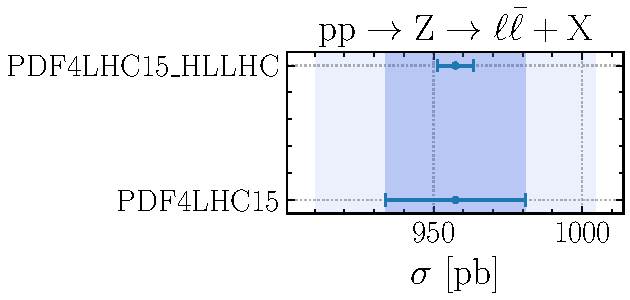
\includegraphics[width=0.32\textwidth]{plots/LHCpheno/NNPDF_DY_14TEV_40_PHENO-integrated-HLLHC.pdf}
	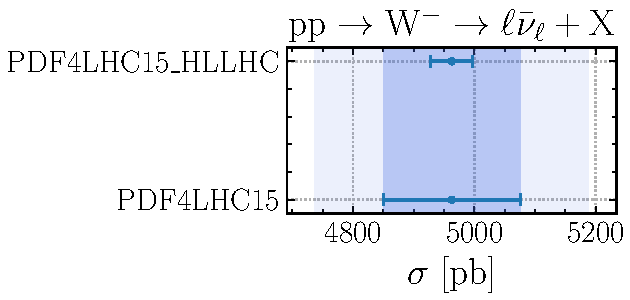
\includegraphics[width=0.32\textwidth]{plots/LHCpheno/NNPDF_WM_14TEV_40_PHENO-integrated-HLLHC.pdf}
	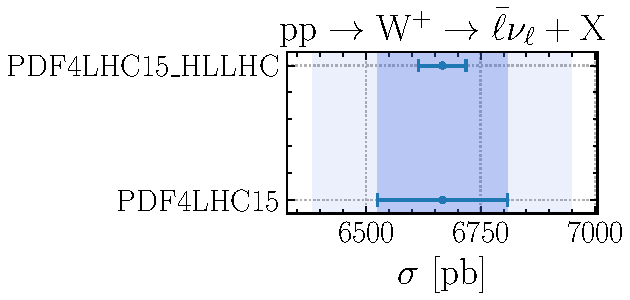
\includegraphics[width=0.32\textwidth]{plots/LHCpheno/NNPDF_WP_14TEV_40_PHENO-integrated-HLLHC.pdf}
	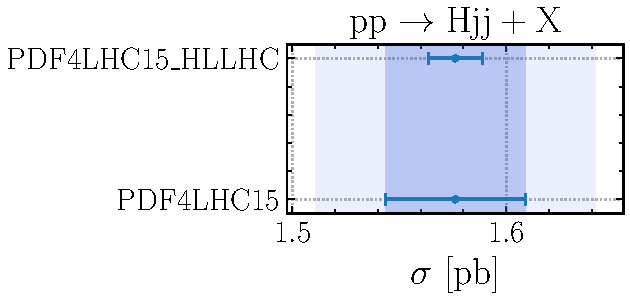
\includegraphics[width=0.32\textwidth]{plots/LHCpheno/NNPDF_HVBF_14TEV_40_PHENO-integrated-HLLHC.pdf}
	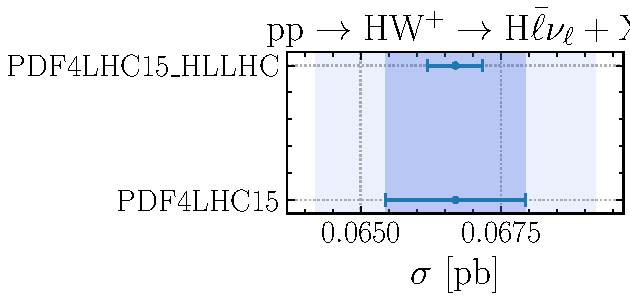
\includegraphics[width=0.32\textwidth]{plots/LHCpheno/NNPDF_HWP_14TEV_40_PHENO-integrated-HLLHC.pdf}
	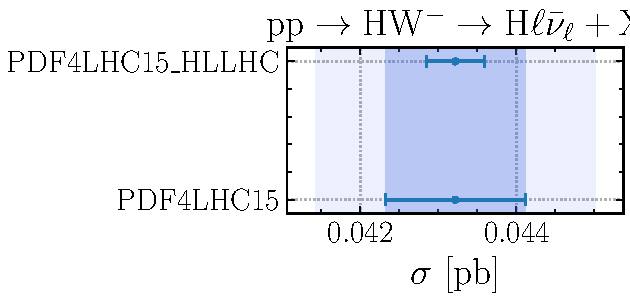
\includegraphics[width=0.32\textwidth]{plots/LHCpheno/NNPDF_HWM_14TEV_40_PHENO-integrated-HLLHC.pdf}
	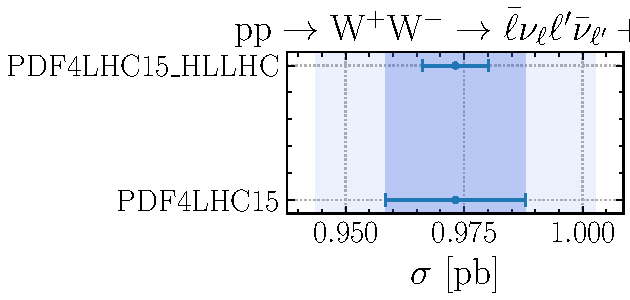
\includegraphics[width=0.32\textwidth]{plots/LHCpheno/NNPDF_WPWM_14TEV_40_PHENO-integrated-HLLHC.pdf}
	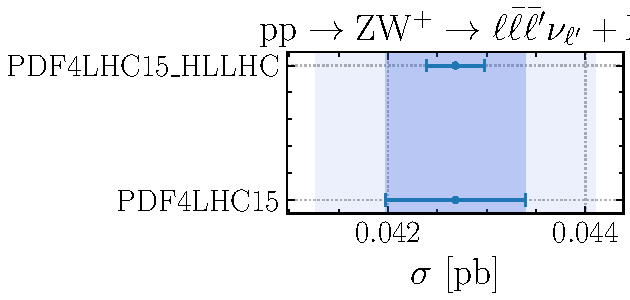
\includegraphics[width=0.32\textwidth]{plots/LHCpheno/NNPDF_WPZ_14TEV_40_PHENO-integrated-HLLHC.pdf}
	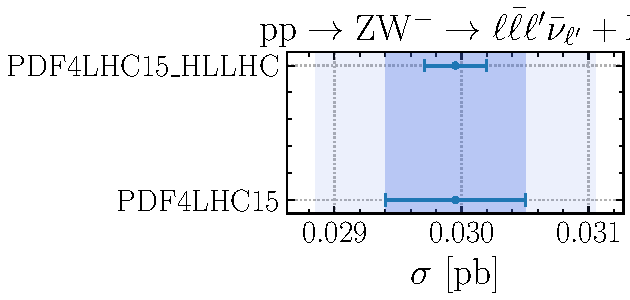
\includegraphics[width=0.32\textwidth]{plots/LHCpheno/NNPDF_WMZ_14TEV_40_PHENO-integrated-HLLHC.pdf}
	\caption{The same LHC fiducial cross-sections as in Fig.~\ref{fig:NNPDF40_pheno_integrated},
          now comparing the PDF4LHC15 baseline predictions with those based
          on the PDFs including HL-LHC pseudo-data from~\cite{AbdulKhalek:2018rok}.
          %
          Specifically, we consider the HL-LHC PDF projections
          from ``Scenario B'', corresponding to an intermediate scenario for the expected reduction
          of systematic uncertainties. }
	\label{fig:HLLHC_pheno_integrated}
\end{figure*}
%%%%%%%%%%%%%%%%%%%%%%%%%%%%%%%%%%%%%%%%%%%%%%%%%%%%%%%%%%%%%%%%%%%%%%%%

Here we revisit the phenomenology studies as in
Sec.~\ref{sec:pheno} but using the High-Luminosity LHC (HL-LHC) PDF 
from~\cite{AbdulKhalek:2018rok}.
%
Such comparisons present a complementary study to the impact seen both at the PDF 
and prediction level shown in Sec.~\ref{sec:pheno}. The PDF constraints from the 
FPF and HL-LHC experiments are fully orthogonal in that the former have the very 
important property that possible contamination from new physics on the PDF fits 
can be completely ignored, since this process is driven by $Q^2$ values outside 
the possible presence of BSM physics.
%
Specially, should anomalies be revealed at the HL-LHC, having the fully independent
validation of the large-$x$ PDFs provided by the FPF would be extremely valuable 
for its interpretation.

In Fig.~\ref{fig:HLLHC_pheno_integrated} The same LHC fiducial cross-sections as in Fig.~\ref{fig:NNPDF40_pheno_integrated},
now comparing the PDF4LHC15 baseline predictions with those based
on the PDFs including HL-LHC pseudo-data from~\cite{AbdulKhalek:2018rok}.
%
Specifically, we consider the HL-LHC PDF projections
from ``Scenario B'', corresponding to an intermediate scenario for the expected reduction
of systematic uncertainties.
 %
Concerning the fiducial cross-sections, a significant reduction in PDF uncertainties
is seen, reaching up to a factor of four for processes involving single boson productions. 
Such a significant decrease in the PDF uncertainties is also observed at the differential
level.


